%\documentclass[aspectratio=169,notes]{beamer}       % print frame + notes
%\documentclass[aspectratio=169][notes=only]{beamer}   % only notes
\documentclass[aspectratio=169]{beamer}              % only frames

%\setbeameroption{hide notes}
\setbeamertemplate{note page}[plain]

\mode<presentation> {
%  \usetheme{Warsaw}
	\usetheme{metropolis} 
}

\usepackage{pgfpages}

\setbeamertemplate{footline}[frame number]
\addtocounter{framenumber}{-1}

%\usepackage{ucs}
\usepackage[utf8]{inputenc}
\usepackage[czech]{babel}
%\usepackage{palatino}
\usepackage{graphicx}
\usepackage{listings}
\usepackage{fontawesome}
\usepackage{multirow}

\title[Open Source Development Course]{Open Source Development Course\\ \small Lifecycle of open source contribution, project management}
\author{Vojtěch Trefný\\ \small \texttt{vtrefny@redhat.com}\\}
\date{16.~3.~2022}
 \institute{\faTwitter\, \href{https://twitter.com/vojtechtrefny}{twitter.com/vojtechtrefny} \\ \faGithub\, \href{https://github.com/vojtechtrefny}{github.com/vojtechtrefny} \\ \faGitlab\ \href{https://gitlab.com/vtrefny}{gitlab.com/vtrefny}}

\begin{document}

{\setbeamertemplate{footline}{} 
\begin{frame}
\titlepage
\end{frame}
}

\newcommand*\openquote{\makebox(25,-22){\scalebox{5}{``}}}
\newcommand*\closequote{\makebox(25,-22){\scalebox{5}{''}}}

%%%%%%%%%%%%%%%%%%%%%%%%%%%%%%%%%%%%%%%%%%%%%%%%%%%%%%%%%%%%%%%%%%

\section{Open source contribution lifecycle}

\begin{frame}
	\frametitle{Contribution lifecycle}
	
\begin{columns}
\begin{column}{0.5\textwidth}
   	\begin{block}{\color{orange}{1. Issue}}
   		\vspace{1mm}
Reporting your own bug or RFE or picking an existing issue to work on.
	\end{block}
	\begin{block}{\color{orange}{2. Fork}}
   		\vspace{1mm}
Getting the code to work in your own ``workspace''.
     \end{block}
         \begin{block}{\color{orange}{3. Development}}
   		\vspace{1mm}
The easy part :-)\\~
     \end{block}
     
\end{column}
\begin{column}{0.5\textwidth} 
\begin{block}{\color{orange}{4. Tests}}
   		\vspace{1mm}
CI test results and/or manual testing.\\~
     \end{block}
      \begin{block}{\color{orange}{5. Code review}}
   		\vspace{1mm}
Code review by the maintainer and making changes.
     \end{block}
      \begin{block}{\color{orange}{6. Rebase \& merge}}
   		\vspace{1mm}
Adjust to the current master and merging the changes.
     \end{block}
\end{column}
\end{columns}
\end{frame}

\begin{frame}
	\frametitle{Disclaimer}
	
\begin{columns}
\begin{column}{0.5\textwidth}
	\begin{block}{}
		\begin{itemize}
			\item These topics are usually different for each project, always check contributor guidelines for specific use cases and workflows.
			\item This part of the lecture is highly based on GitHub workflow. It applies to similar services like GitLab as well, but projects that don't use these ``advanced'' code hosting services and rely mostly on emails and mailing list are very different.
		\end{itemize}
	\end{block}
\end{column}

\begin{column}{0.5\textwidth}
	\begin{figure}[ht!]
	\begin{center}
  	  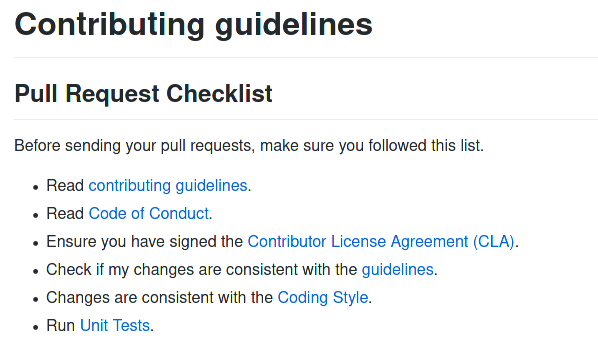
\includegraphics[width=0.95\textwidth]{img/gh-contributor-guidelines.png}
	\end{center}
	\end{figure}
\end{column}
\end{columns}

\tiny\url{https://github.com/tensorflow/tensorflow/blob/master/CONTRIBUTING.md}
\end{frame}

\begin{frame}
	\frametitle{Issue trackers}
	
	\begin{block}{}
		\begin{itemize}
			\item Code hosting services like GitHub and GitLab offer integrated issues trackers.
			\item Some projects use separate tools like Bugzilla or JIRA for tracking bugs and RFEs.
		\end{itemize}
	\end{block}

	\begin{block}{}
		\begin{itemize}
			\item Issues allow you to discuss the bug/feature with other developers and users.
			\item Starting with an issue or bug report is not necessary but not doing that increases the risk of your contribution being ignored or rejected.
		\end{itemize}
	\end{block}
\end{frame}

\begin{frame}
	\frametitle{GitHub Issues}
	
	\begin{block}{}
		\begin{itemize}
			\item GitHub helps first-time contributors to discover \emph{good first issues} to help the project with.
		\end{itemize}
	\end{block}
	
	\begin{figure}[ht!]
	\begin{center}
  	  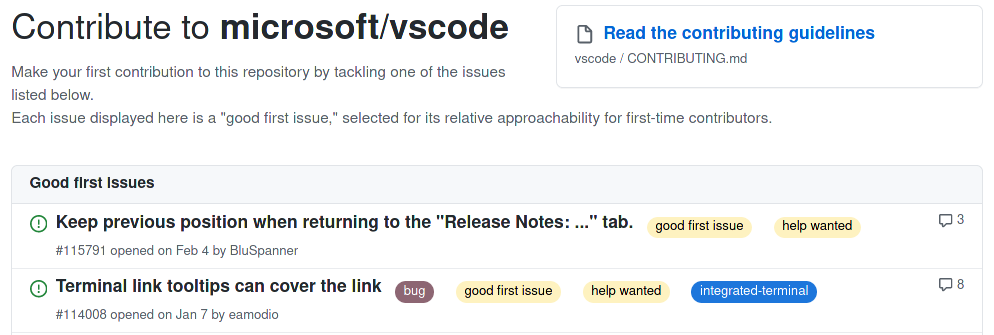
\includegraphics[width=0.8\textwidth]{img/gh-good-first-issue.png}
	\end{center}
	\end{figure}


\tiny{\url{https://github.com/microsoft/vscode/contribute}}
\end{frame}

\begin{frame}
	\frametitle{GitHub Issues}
	
	\begin{columns}
\begin{column}{0.45\textwidth}
	\begin{figure}[ht!]
	\begin{center}
  	  
\includegraphics[width=0.9\textwidth]{img/gh-issue-assign.png}
	\end{center}
	\end{figure}
\end{column}
\begin{column}{0.05\textwidth}
\begin{center}
\large$\rightarrow$
\end{center}
\end{column}
\begin{column}{0.45\textwidth}
\begin{figure}[ht!]
	\begin{center}
  	  
\includegraphics[width=0.9\textwidth]{img/gh-issue-assigned.png}
	\end{center}
	\end{figure}
\end{column}
\end{columns}
	
\begin{block}{}
		\begin{itemize}
			\item Do not forget to assign the issue to yourself to let others know you are working on it.
		\end{itemize}
	\end{block}

\end{frame}

\begin{frame}
	\frametitle{Fork}
	
	\begin{block}{}
		\begin{itemize}
			\item A fork is your own ``copy'' of the upstream repository.
			\item On GitHub (and similar sites) having a fork is needed to be able to open a \emph{pull request} later.
		\end{itemize}
	\end{block}
	
	\begin{columns}
\begin{column}{0.30\textwidth}
	\begin{figure}[ht!]
	\begin{center}
  	  
\includegraphics[width=0.9\textwidth]{img/gh-fork-3.png}
	\end{center}
	\end{figure}
\end{column}

\begin{column}{0.03\textwidth}
\begin{center}
$\rightarrow$
\end{center}
\end{column}

\begin{column}{0.30\textwidth}
\begin{figure}[ht!]
	\begin{center}
  	  
\includegraphics[width=0.9\textwidth]{img/gh-fork-1.png}
	\end{center}
\end{figure}
\end{column}

\begin{column}{0.03\textwidth}
\begin{center}
$\rightarrow$
\end{center}
\end{column}

\begin{column}{0.30\textwidth}
\begin{figure}[ht!]
	\begin{center}
  	  
\includegraphics[width=0.9\textwidth]{img/gh-fork-2.png}
	\end{center}
\end{figure}
\end{column}
\end{columns}

\end{frame}

\begin{frame}[fragile]
	\frametitle{Fork}
	
	\begin{block}{}
		\begin{itemize}
			\item It's a good practice to clone the upstream repository and add your fork as a second \emph{remote}.
			\item This will help you when \emph{rebasing} to the latest upstream version.
		\end{itemize}
	\end{block}
	
\begin{lstlisting}[frame=none, basicstyle=\ttfamily\small, columns=fullflexible, keepspaces=true]
$ git remote -v
origin  git@github.com:rhinstaller/dasbus.git (fetch)
origin  git@github.com:rhinstaller/dasbus.git (push)
vtrefny_GH      git@github.com:vojtechtrefny/dasbus.git (fetch)
vtrefny_GH      git@github.com:vojtechtrefny/dasbus.git (push)
\end{lstlisting}

\end{frame}

\begin{frame}[fragile]
	\frametitle{Pull request}
	
	\begin{block}{}
		\begin{itemize}
			\item After committing your changes, simply push them to your fork and open a \emph{pull request} (in GitLab terminology a \emph{merge request}) using the link provided by the \emph{git push hook}.
		\end{itemize}
	\end{block}
	
	\begin{lstlisting}[frame=none, basicstyle=\ttfamily\small, columns=fullflexible, keepspaces=true]
$ git push vtrefny_GH master_my-feature
...
remote: 
remote: Create a pull request for 'master_my-feature' on GitHub by visiting:
remote:      https://github.com/vojtechtrefny/dasbus/pull/new/master_my-feature
remote: 
To github.com:vojtechtrefny/dasbus.git
 * [new branch]      master_my-feature -> master_my-feature
\end{lstlisting}

\end{frame}

\begin{frame}[fragile]
	\frametitle{Pull request}
	
	\begin{center}
  	  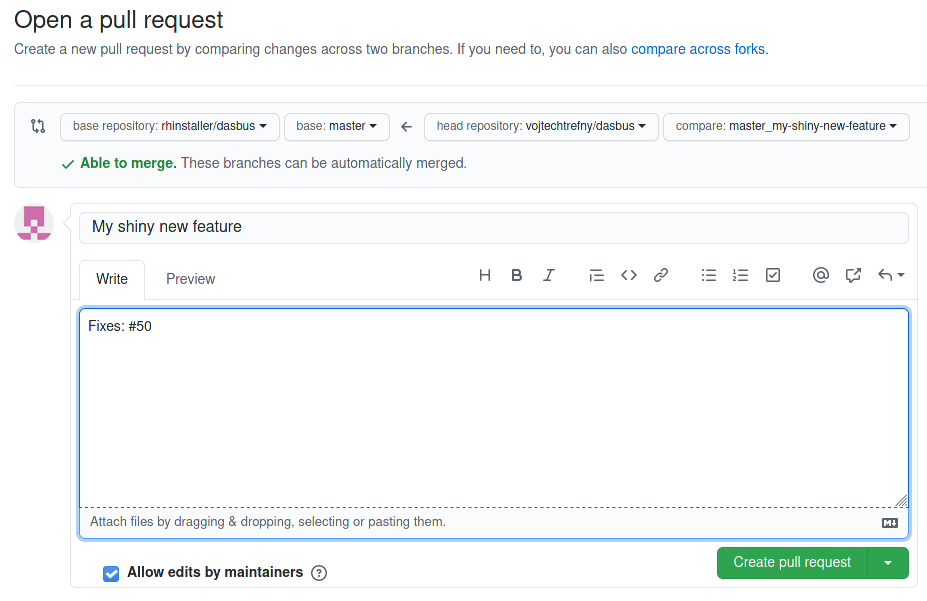
\includegraphics[width=0.8\textwidth]{img/gh-open-pr.png}
	\end{center}
\end{frame}

\begin{frame}
	\frametitle{Automated tests}
	
\begin{block}{}
		\begin{itemize}
			\item If the project has CI configured, automated tests will run on your PR.
			\item Multiple different tests and checks, including static analysis and builds, may be applied.
			\item Some projects can reject or ignore PRs with failing tests.
			\item More about tests and CI next week.
		\end{itemize}
	\end{block}
	
\begin{columns}

\begin{column}{0.4\textwidth}
\begin{figure}[ht!]
	\begin{center}
  	  
\includegraphics[width=\textwidth]{img/gh-ci-success.png}
	\end{center}
\end{figure}
\end{column}

\begin{column}{0.4\textwidth}
\begin{figure}[ht!]
	\begin{center}
  	  
\includegraphics[width=\textwidth]{img/gh-ci-fail.png}
	\end{center}
\end{figure}
\end{column}
\end{columns}

\end{frame}

\begin{frame}
	\frametitle{Code review}
	
\begin{block}{}
		\begin{itemize}
			\item During code review, other project contributors and maintainers will review your changes to either approve or reject them or request changes.
			\item When changes are requested you can either change the existing commits or add \emph{fix} commits that will be \emph{squashed} later.
			\item At least one \emph{approve} review from a project maintainer is usually needed for the change to be merged.
			\item For more complicated changes, long back and forth reviews with multiple discussions are not uncommon.
		\end{itemize}
\end{block}

\begin{columns}
\begin{column}{0.4\textwidth}
\begin{figure}[ht!]
	\begin{center}
  	  
\includegraphics[width=0.7\textwidth]{img/gh-reviewers.png}
	\end{center}
\end{figure}
\end{column}

\begin{column}{0.4\textwidth}
\begin{figure}[ht!]
	\begin{center}
  	  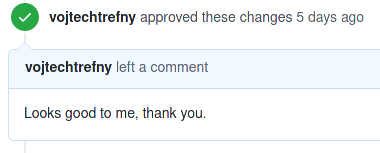
\includegraphics[width=0.8\textwidth]{img/gh-review-approve.png}
	\end{center}
\end{figure}
\end{column}
\end{columns}

\end{frame}

\begin{frame}
	\frametitle{Code review}
	
\begin{figure}[ht!]
	\begin{center}
  	  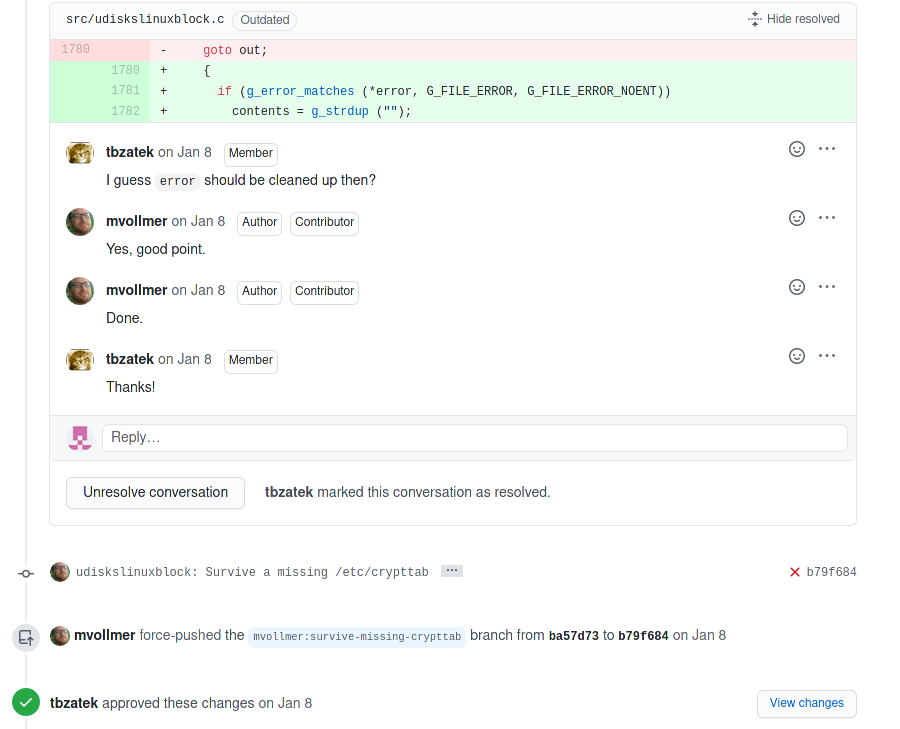
\includegraphics[width=0.65\textwidth]{img/gh-review.png}
	\end{center}
\end{figure}
	
\end{frame}

\begin{frame}
	\frametitle{Rebase \& merge}
	
\begin{block}{}
		\begin{itemize}
			\item If the CI and review phases take a long time, merge conflicts can occur, especially in more active projects.
			\item \texttt{git} can solve some conflicts automatically, but you might need to resolve some manually.
			\item Pull requests with conflicts cannot be merged.
		\end{itemize}
\end{block}

\begin{figure}[ht!]
	\begin{center}
  	  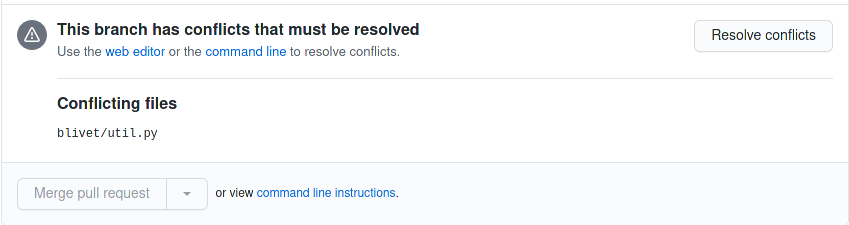
\includegraphics[width=0.7\textwidth]{img/gh-merge-conflict.png}
	\end{center}
\end{figure}

\end{frame}

\begin{frame}
	\frametitle{Release}
	
\begin{block}{}
		\begin{itemize}
			\item After the contribution is merged, it should be included in the next release.
			\item Depending on project release schedule and development state, this might happen immediately or take few weeks or months.
			\item At some stages, projects might not accept other contributions than bug fixes and new features might be accepted only for development branches/releases or not at all.
		\end{itemize}
\end{block}
\begin{figure}[ht!]
	\begin{center}
  	  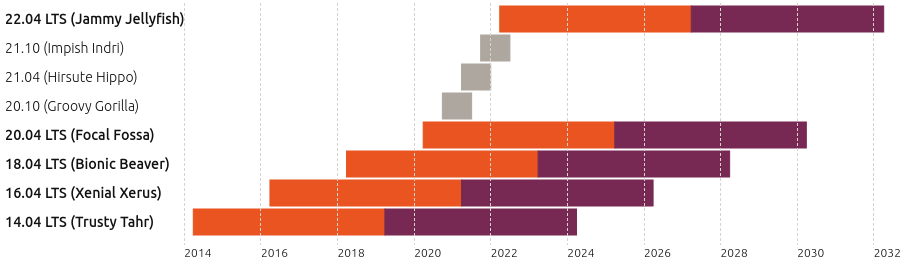
\includegraphics[width=0.7\textwidth]{img/ubuntu-releases.png}
	\end{center}
\end{figure}

\end{frame}

\begin{frame}
	\frametitle{Release life cycle}
	
\begin{columns}
\begin{column}{0.5\textwidth}
   	\begin{block}{\color{orange}{1. Planning}}
   		\vspace{1mm}
Gathering use cases. Product and objectives definition.
	\end{block}
	\begin{block}{\color{orange}{2. Pre-Alpha}}
   		\vspace{1mm}
Early development, usually not meant for public.
     \end{block}
         \begin{block}{\color{orange}{3. Alpha/Beta}}
   		\vspace{1mm}
Pre-releases for testing purposes and early adopters.
     \end{block}
     
\end{column}
\begin{column}{0.5\textwidth} 
\begin{block}{\color{orange}{4. Release candidate (RC)}}
   		\vspace{1mm}
Candidate for the stable release.\\~
     \end{block}
      \begin{block}{\color{orange}{5. Stable release}}
   		\vspace{1mm}
Stable release targeted for end-users.
     \end{block}
      \begin{block}{\color{orange}{6. Mature project/Maintenance}}
   		\vspace{1mm}
Maintenance and bug fixing. EOL or continuous development.
     \end{block}
\end{column}
\end{columns}

\end{frame}

\begin{frame}
	\frametitle{Fedora release cycle}

\begin{center}
\begin{tabular}{l c c}
    Rawhide starts Fedora Linux 37 development & 2022-02-08 \\
    Proposal submission deadline (System Wide Changes) & 2022-06-28 \\
    Proposal submission deadline (Self Contained Changes) & 2022-07-19 \\
    Completion deadline (testable) & 2022-08-09  \\
    Branch Fedora Linux 37 from Rawhide & 2022-08-09 \\
    Change Checkpoint: 100 \% Code Complete Deadline & 2022-08-23  \\
    Beta Release & 2022-09-13 \\
    Final Freeze  & 2022-10-04 \\
    Final & 2022-10-18 \\
    Rawhide starts Fedora Linux 38 development  &  2022-08-09 \\
    Fedora Linux 37 EOL  & 2023-11-14 \\
\end{tabular}
\end{center}

\tiny{\url{https://fedorapeople.org/groups/schedule/f-37/f-37-key-tasks.html}}
\end{frame}

\begin{frame}
	\frametitle{Fedora release cycle}

\begin{center}
\begin{tabular}{c l c c}
  \multirow{3}{*}{\color{orange}Planning} & Rawhide starts Fedora Linux 37 development & 2022-02-08 \\
   & Proposal submission deadline (System Wide Changes) & 2022-06-28 \\
   & Proposal submission deadline (Self Contained Changes) & 2022-07-19 \\ \hline
  \multirow{2}{*}{\color{orange}Pre-alpha}   & Completion deadline (testable) & 2022-08-09  \\
   & Branch Fedora Linux 37 from Rawhide & 2022-08-09 \\ \hline
   \multirow{2}{*}{\color{orange}Alpha/Beta}  & Change Checkpoint: 100 \% Code Complete Deadline & 2022-08-23  \\
   & Beta Release & 2022-09-13 \\ \hline
  \color{orange}RC  & Final Freeze  & 2022-10-04 \\ \hline
  \color{orange}Stable release & Final & 2022-10-18 \\ \hline
  \multirow{2}{*}{\color{orange}Maintenance}  & Rawhide starts Fedora Linux 38 development  &  2022-08-09 \\
   & Fedora Linux 37 EOL  & 2023-11-14 \\
\end{tabular}
\end{center}
\end{frame}


\section{Software dependencies}

\begin{frame}
	\frametitle{Software dependencies}
	
	\begin{block}{}
		\begin{itemize}
			\item Using existing libraries and tools can save a lot of time when building a new project.
			\item Managing third party dependencies can be tricky, but when done properly, it's better and safer than writing code from scratch.
			\item When working with dependencies it's crucial to make sure your
			\begin{itemize}
				\item code is up to date,
				\item system is secure,
				\item service/project works as intended.
			\end{itemize}
		\end{itemize}
	\end{block}


\end{frame}

\begin{frame}
	\frametitle{Types of dependencies}
\begin{columns}
\begin{column}{0.5\textwidth}
   	\begin{center}{\color{orange}{Direct dependencies}}
   		\vspace{1mm}\\
Libraries that your code directly depends upon. These require some effort to control but are sort of manageable.
	\end{center}
     
\end{column}
\begin{column}{0.5\textwidth} 
\begin{center}{\color{orange}{Transitive dependencies}}
   		\vspace{1mm}\\
Dependencies of the dependencies.\\Usually quite hard to control.\\~
     \end{center}
\end{column}
\end{columns}

\vspace{10mm}

\begin{columns}
\begin{column}{0.25\textwidth}
\end{column}

\begin{column}{0.5\textwidth}
\begin{center}{\color{orange}{Third party dependencies}}
   		\vspace{1mm}\\
A special kind. These are the dependencies that you don't own and that are not part of your organization. 
     \end{center}
\end{column}

\begin{column}{0.25\textwidth}
\end{column}
\end{columns}

\end{frame}

\begin{frame}[fragile]
	\frametitle{Transitive dependencies}
	
\begin{columns}
\begin{column}{0.5\textwidth}
	\begin{figure}[ht!]
	\begin{center}
  	  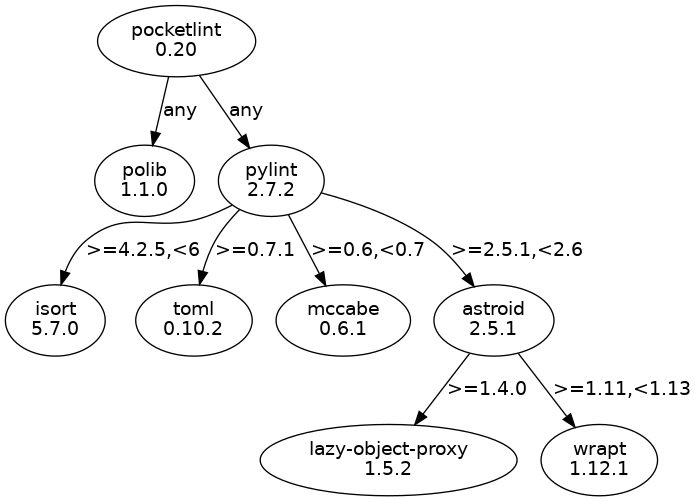
\includegraphics[width=\textwidth]{img/dependencies.png}
	\end{center}
	\end{figure}
\end{column}
\begin{column}{0.5\textwidth}
\begin{lstlisting}[frame=none, basicstyle=\ttfamily\small, escapechar=$, columns=fullflexible, keepspaces=true]
pocketlint
  - polib [Any]
  - pylint [Any]
    - astroid [>=2.5.1,<2.6]
      - lazy-object-proxy [>=1.4.0]
      - wrapt [>=1.11,<1.13]
    - isort [>=4.2.5,<6]
    - mccabe [>=0.6,<0.7]
    - toml [>=0.7.1]
\end{lstlisting}
\end{column}
\end{columns}
\end{frame}

\subsection{Dependency management}

\begin{frame}
	\frametitle{Dependency management}
	
	\begin{block}{}
		\begin{itemize}
			\item Dependencies are usually managed using a project or language-specific tool which takes care of resolving and pulling in third-party dependencies, including transitive dependencies.
			\item Dependencies can be downloaded during the build (for build and built-in dependencies) or project or service installation or deployment.
			\item Dependencies can be available either in a public or project-specific repository.
			\item Some dependency management can also detect required dependencies from the code.
		\end{itemize}
	\end{block}
\end{frame}

\begin{frame}
	\frametitle{Package repositories}
	
\begin{columns}
	\begin{column}{0.5\textwidth}
		\begin{itemize}
			\item Different package repositories exist for different programming languages or frameworks:
			\begin{itemize}
				\item Python Package Index (PyPI) for Python with \texttt{pip} tool.\footnotemark
				\item Rust crate registry for Rust with \texttt{cargo} tool.\footnotemark
				\item Node Package Manager (NPM) with \texttt{npm} tool.\footnotemark
			\end{itemize}
		\end{itemize}
	\end{column}
	\begin{column}{0.5\textwidth}
	\begin{figure}[ht!]
	\begin{center}
  	  
\includegraphics[width=\textwidth]{img/pypi.png}
	\end{center}
	\end{figure}
	\end{column}
\end{columns}

\footnotetext[1]{\tiny\url{https://pypi.org}}
\footnotetext[2]{\tiny\url{https://crates.io}}
\footnotetext[3]{\tiny\url{https://www.npmjs.com}}
\end{frame}

\begin{frame}[fragile]
	\frametitle{PyPI}
	
\begin{columns}
\begin{column}{0.4\textwidth}
\begin{figure}[ht!]
	\begin{center}
  	  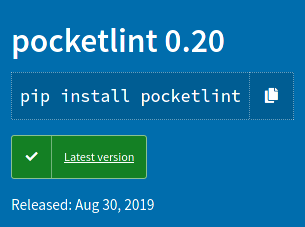
\includegraphics[width=5cm]{img/pocketlint.png}
	\end{center}
	\end{figure}
\end{column}
\begin{column}{0.6\textwidth}
\begin{lstlisting}[frame=none, basicstyle=\ttfamily\small, escapechar=$, columns=fullflexible, keepspaces=true]
setup(
   name='pocketlint', version='0.20',
   description='Support for running ...
   url='https://github.com/...
   install_requires=['pylint', 'polib'],
   ...
)
\end{lstlisting}
\end{column}
\end{columns}
\end{frame}

\begin{frame}[fragile]
	\frametitle{PyPI}
	
\begin{lstlisting}[frame=none, basicstyle=\ttfamily\small, columns=fullflexible, keepspaces=true]
$ pip install pocketlint
Collecting pocketlint
  Using cached pocketlint-0.20-py3-none-any.whl (32 kB)
Collecting pylint
  Using cached pylint-2.7.2-py3-none-any.whl (342 kB)
Collecting polib
  Using cached polib-1.1.0-py2.py3-none-any.whl (25 kB)
...
Collecting astroid<2.6,>=2.5.1
  Using cached astroid-2.5.1-py3-none-any.whl (222 kB)
Collecting wrapt<1.13,>=1.11
  Using cached wrapt-1.12.1.tar.gz (27 kB)
Collecting lazy-object-proxy>=1.4.0
  Using cached lazy_object_proxy-1.5.2-cp39-cp39-manylinux1_x86_64.whl (53 kB)
Installing collected packages: mccabe, isort, toml, wrapt, lazy-object-proxy, 
	astroid, pylint, polib, pocketlint
\end{lstlisting}
	
\end{frame}



\section{What could go wrong?}

\begin{frame}
	\frametitle{Missing package that ``broke'' the Internet}
	
	\begin{figure}[ht!]
	\begin{center}
  	  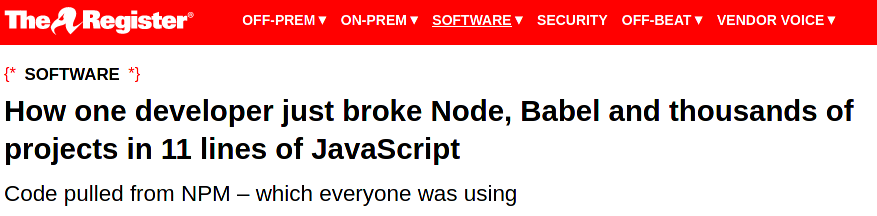
\includegraphics[width=12cm]{img/deps-npm-2.png}
	\end{center}
	\end{figure}
	
	\begin{block}{}
		In 2016 Azer Koçulu unpublished more than 250 of his packages from NPM, including a very popular \texttt{left-pad} package which many big JavaScript projects (including React) depended on.\footnotemark~\footnotemark
	\end{block}

\footnotetext[4]{\tiny\url{https://www.theregister.com/2016/03/23/npm_left_pad_chaos/}}
\footnotetext[5]{\tiny\url{https://blog.npmjs.org/post/141577284765/kik-left-pad-and-npm}}
\end{frame}

\begin{frame}
	\frametitle{What could go wrong?}
\begin{columns}
\begin{column}{0.5\textwidth}
   	\begin{block}{\color{orange}{Security vulnerabilities (CVE)}}
   		\vspace{1mm}
   		\small\emph{Old versions of dependencies with unfixed vulnerabilities.}
	\end{block}
	\begin{block}{\color{orange}{Version conflicts}}
   		\vspace{1mm}
   		\small\emph{Circular dependencies and dependency hell.}
     \end{block}
         \begin{block}{\color{orange}{Missing/removed dependency}}
   		\vspace{1mm}
   		\small\emph{Packages removed from repositories.}
     \end{block}
     
\end{column}
\begin{column}{0.5\textwidth}
\begin{block}{\color{orange}{API/ABI changes}}
   		\vspace{1mm}
   		\small\emph{New versions with backwards-incompatible changes.}
     \end{block}
      \begin{block}{\color{orange}{Broken third-party dependencies}}
   		\vspace{1mm}
   		\small\emph{Bugs in code that is not under your control.}
     \end{block}
      \begin{block}{\color{orange}{License conflicts}}
   		\vspace{1mm}
   		\small\emph{Incompatible open source licenses.}
     \end{block}
\end{column}
\end{columns}
\end{frame}

\begin{frame}
	\frametitle{Version conflicts}
	

\begin{columns}
\begin{column}{0.5\textwidth}

	\begin{block}{}
		\begin{itemize}
			\item Two or more packages depending on the same package but a different version.
			\item Unsolvable if multiple versions of the same package cannot be installed together.
			\item Sometimes referred to as ``dependency hell'' (especially in relation to distributions and solving of dependencies during package installation or upgrade).
		\end{itemize}
	\end{block}

\end{column}

\begin{column}{0.5\textwidth}
	\begin{figure}[ht!]
	\begin{center}
  	  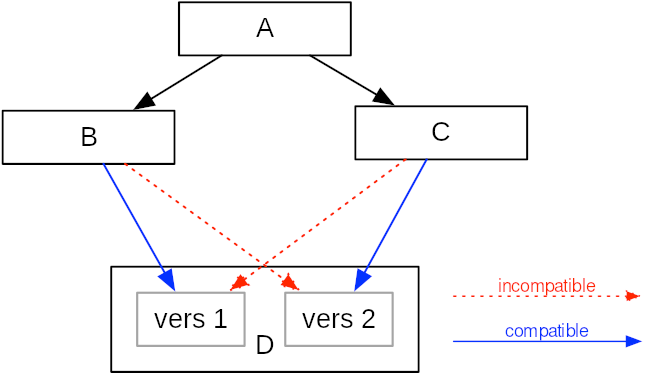
\includegraphics[width=\textwidth]{img/dependency-hell.png}
	\end{center}
	\end{figure}
\end{column}
\end{columns}

\tiny{\url{https://research.swtch.com/version-sat}}
\end{frame}

\begin{frame}
	\frametitle{API/ABI stability}
	
	\begin{columns}

\begin{column}{0.5\textwidth}
	\begin{figure}[ht!]
	\begin{center}
  	  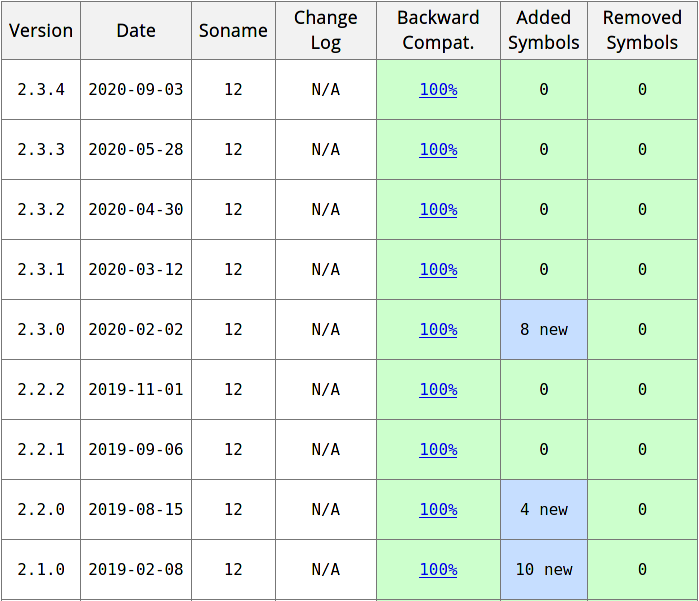
\includegraphics[width=\textwidth]{img/abi.png}
	\end{center}
	\end{figure}
\end{column}

\begin{column}{0.5\textwidth}
	\begin{block}{}
		\begin{itemize}
			\item Backward incompatible changes should happen only in major versions.
			\item Keeping compatibility with multiple API versions require additional code and tests.
			\item For compiled languages with dynamic libraries, ABI stability is also crucial. Rebuilding the entire project because of a single dependency ABI change might not be possible.
		\end{itemize}
	\end{block}

\end{column}
\end{columns}
\tiny{\url{https://abi-laboratory.pro/?view=timeline&l=cryptsetup}}
\end{frame}

\begin{frame}
	\frametitle{CVEs}
	
	\begin{columns}
\begin{column}{0.6\textwidth}

	\begin{block}{}
		\begin{itemize}
			\item Both security vulnerabilities and ``normal'' bugs in dependencies can easily compromise your application.
			\item Recent bugs like Heartbleed\footnotemark in OpenSSL showed that many essential opensource libraries are understaffed and have many unfixed vulnerabilities.
			\item Bundled dependencies needs to be closely monitored for CVEs and quickly updated.
		\end{itemize}
	\end{block}

\end{column}

\begin{column}{0.4\textwidth}
	\begin{figure}[ht!]
	\begin{center}
  	  
\includegraphics[width=0.65\textwidth]{img/heartbleed.png}
	\end{center}
	\end{figure}
\end{column}
\end{columns}

\footnotetext[6]{\tiny{\url{https://heartbleed.com/}}}
\end{frame}

\begin{frame}
	\frametitle{Log4Shell}
	
\begin{columns}
\begin{column}{0.68\textwidth}

		\begin{itemize}
			\item Security vulnerability (\emph{remote code execution}) in Log4j, Java logging framework, discovered in November 2021 (disclosed in December). \footnotemark~\footnotemark
		\end{itemize}
\end{column}

\begin{column}{0.25\textwidth}
	\begin{figure}[ht!]
	\begin{center}
  	  
\includegraphics[width=0.95\textwidth]{img/log4j.png}
	\end{center}
	\end{figure}
\end{column}
\end{columns}

		\begin{itemize}
			\item Affected many projects including AWS, Cloudflare and iCloud. Up to 93 \% of cloud environments were affected.
			\item Similarly to Heartbleed, Log4Shell again draw attention to open source projects that are heavily depended on but not properly staffed and financed.\footnotemark
			\item Log4Shell being a way smaller project than OpenSSL and often being bundled in biggers project also showed how hard is to track and manage dependencies.
		\end{itemize}

\footnotetext[7]{\tiny{\url{https://www.nukib.cz/cs/infoservis/hrozby/1781-upozorneni-na-zranitelnost-apache-log4j-log4shell/}}}
\footnotetext[8]{\tiny{\url{https://www.nukib.cz/cs/infoservis/hrozby/1785-nukib-vydava-reaktivni-opatreni-v-souvislosti-se-zranitelnosti-log4shell/}}}
\footnotetext[9]{\tiny{\url{https://gizmodo.com/after-log4j-open-source-software-is-now-a-national-sec-1848356403}}}

\end{frame}

\begin{frame}
	\frametitle{Dead and abandoned projects}
	
	\begin{columns}
\begin{column}{0.55\textwidth}

	\begin{block}{}
		\begin{itemize}
			\item Especially smaller projects can very quickly become unmaintained or abandoned.
			\item Upstream source can be even completely lost after service or domain expiration.
			\item Upstream can move to a different fork or cease to exist without replacement.
			\item For actively maintained projects, older stable versions can be abandoned long before your product EOL.
		\end{itemize}
	\end{block}

\end{column}

\begin{column}{0.45\textwidth}
	\begin{figure}[ht!]
	\begin{center}
  	  
\includegraphics[width=1\textwidth]{img/dead-project.png}
	\end{center}
	\end{figure}
\end{column}
\end{columns}

\vspace{3mm}
\tiny{\url{https://www.open-fcoe.org/git}}
\end{frame}

\begin{frame}
	\frametitle{License compatibility}
	
	\begin{block}{}
		\begin{itemize}
			\item Not all free and/or opensource licenses are compatible.
			\item Some licenses require the result to be released under the ``stronger'' license.
			\item Different rules might apply for different types of dependencies -- copying code vs. linking vs. calling.
			\item More about licenses in the \emph{Open source licenses} lecture.
		\end{itemize}
	\end{block}
	
	
\end{frame}

\begin{frame}
	\frametitle{License compatibility}
	
	\begin{figure}[ht!]
	\begin{center}
  	  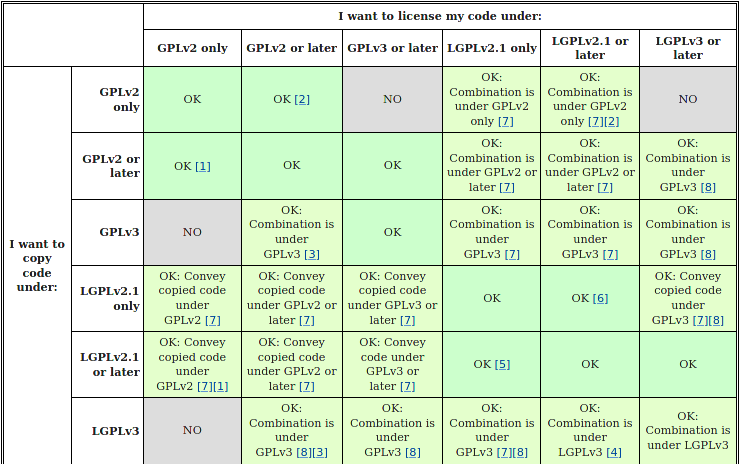
\includegraphics[width=11cm]{img/license-compatibility.png}
	\end{center}
	\end{figure}

\tiny{\url{https://www.gnu.org/licenses/gpl-faq.html\#AllCompatibility}}
\end{frame}


%%%%%%%%%%%%%%%%%%%%%%%%%%%%%%%%%%%%%%%%%%%%%%%%%%%%%%%%%%%%%%%%%%

\section{Questions}

\begin{frame}
	\frametitle{Questions}

	\begin{center}
	Thank you for your attention.
	\end{center}

\vspace{0.5cm}

	\begin{center}
	\color{blue}{\url{https://github.com/crocs-muni/open-source-development-course}}
	\end{center}
\end{frame}

\end{document}

